\documentclass{beamer}
%\usepackage[T1]{fontenc}
\usepackage[utf8]{inputenc}
%\usepackage{lmodern}  % Use the Latin Modern font family

\usepackage{latexsym,amsmath,xcolor,bm, amssymb, color, tikz, graphicx, amsthm, mathtools}
\usepackage{algorithm}
\usepackage{algorithmic}
\usepackage{hyperref}
\usepackage{float}     
\usepackage{CJKutf8}
\usepackage{multicol}

% Add pgf-pie for pie charts

% Only add if not present
\usepackage{pgf-pie}

\DeclareMathOperator*{\argmax}{arg\,max}
\DeclareMathOperator*{\argmin}{arg\,min}
\DeclareMathOperator{\sign}{sign}
\DeclareMathOperator{\Tr}{Tr}

\makeatletter
\DeclareRobustCommand\onedot{\futurelet\@let@token\@onedot}
\def\@onedot{\ifx\@let@token.\else.\null\fi\xspace}
\def\eg{\emph{e.g}\onedot} 
\def\Eg{\emph{E.g}\onedot}
\def\ie{\emph{i.e}\onedot} 
\def\Ie{\emph{I.e}\onedot}
\def\cf{\emph{c.f}\onedot} 
\def\Cf{\emph{C.f}\onedot}
\def\etc{\emph{etc}\onedot} 
\def\vs{\emph{vs}\onedot}
\def\wrt{w.r.t\onedot} 
\def\dof{d.o.f\onedot}
\def\etal{\emph{et al}\onedot}
\makeatother


\usetheme{Madrid}
\useinnertheme{circles}


\definecolor{ColorUNR}{HTML}{0b2755} 
\usecolortheme[named=ColorUNR]{structure}
%\usecolortheme[named=ColorUNR]{exampleblock}

%\setbeamertemplate{blocks}[rounded][shadow=true]
%\setbeamercolor{block body}{fg=black,bg=white}



%------------------------------------------------------------
%This block of code defines the information to appear in the
%Title page
\title %optional
{Cierre Training Camp 2025}

\subtitle{Ceremonia de Clausura}

%\subtitle{with applications to persuation and lie production}
% \author % (optional)
% {Author Name}

\author[Matias Ramos]{Matias Ramos}

\institute[]{Universidad Tecnológica Nacional - Facultad Regional Santa Fe}
\date[TC 2025]{Training Camp 2025}
\titlegraphic{
\includegraphics[clip,height=2cm,keepaspectratio]{logos/tcarg.jpeg}}

%End of title page configuration block
%------------------------------------------------------------


%------------------------------------------------------------
%The next block of commands puts the table of contents at the 
%beginning of each section and highlights the current section:
\AtBeginSection[]
{
  \begin{frame}
    \frametitle{Outline}
    \tableofcontents[currentsection]
  \end{frame}
}
%------------------------------------------------------------


\begin{document}


%The next statement creates the title page.
\frame{\titlepage}


%------------------------------------------------------------
% Frame de Sponsors, me parece mejor ponerlo al principio
% Antes del índice/contenido

% --- Sponsors Frame 1: Organizador & Diamond Plus ---


% First sponsors frame: Organizador and Diamond Plus
\begin{frame}{Gracias Sponsors!}
    \begin{columns}[t]
        \column{0.5\textwidth}
        \centering
        Organizador\\
        \vspace{0.5cm}
        
\includegraphics[width=1\textwidth,keepaspectratio]{logos/aapc.png}
        
\includegraphics[width=1\textwidth,keepaspectratio]{logos/utn_santafe.png}
        \column{0.5\textwidth}
        \centering
        Diamond Plus\\
        
\includegraphics[width=1\textwidth,keepaspectratio]{logos/GTSlogo.jpeg}
    \end{columns}
\end{frame}

% --- Sponsors Frame 2: Gold & Oro ---

\begin{frame}{Gracias Sponsors!}
    % Platino at the top, full width
    \centering
    Platino\\
    
\includegraphics[width=0.6\textwidth,keepaspectratio]{logos/folder.png}
    
    \vfill
    
    % Gold and Oro at the bottom in two columns
    \begin{columns}[b]
        % Gold column
        \column{0.5\textwidth}
        \centering
        Gold\\
        
\includegraphics[width=0.8\textwidth,keepaspectratio]{logos/neuralsoft.png}
        % Oro column
        \column{0.5\textwidth}
            \centering
        Oro\\
        
\includegraphics[width=0.8\textwidth,keepaspectratio]{logos/jerarquicos.jpg}
    \end{columns}
\end{frame}

% --- Sponsors Frame 3: Aliado ---

\begin{frame}{Gracias Sponsors!}
    \centering
    Aliado\\
    \vspace{1cm}
    
\includegraphics[width=0.6\textwidth,keepaspectratio]{logos/santa_fe_logo_v2.jpg}
\end{frame}


\section{Gracias por venir}

\begin{frame}{Participantes por País}
\begin{center}
\Large
\textbf{¡168 participantes presentes!}

\vspace{0.5cm}

\normalsize
\textbf{Distribución por países:}

\vspace{0.3cm}

\begin{itemize}
\item \textbf{Argentina:} 117 participantes
\item \textbf{Perú:} 14 participantes  
\item \textbf{Chile:} 13 participantes
\item \textbf{Costa Rica:} 8 participantes
\item \textbf{Colombia:} 7 participantes
\item \textbf{México:} 5 participantes
\item \textbf{Uruguay:} 3 participantes
\item \textbf{Brasil:} 1 participante
\end{itemize}

\vspace{0.5cm}

\textbf{¡Gracias por hacer de este evento un éxito internacional!}
\end{center}
\end{frame}

\begin{frame}{Diversidad Regional}
\begin{center}
\Large
\textbf{8 países representados}

\vspace{0.3cm}

% --- Dots Only: Geographically Accurate and All Visible ---

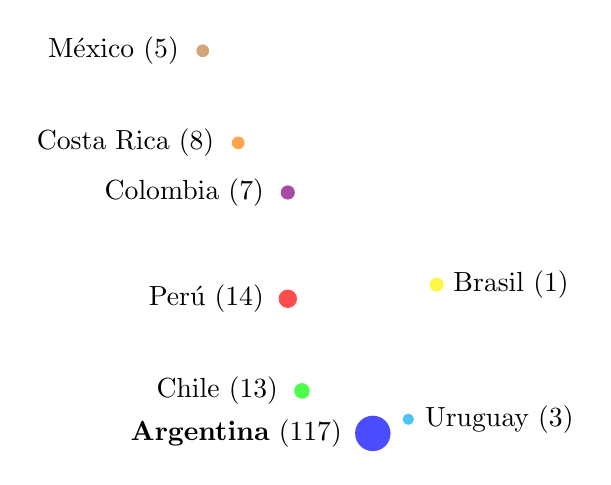
\begin{tikzpicture}[scale=0.9]
  % Argentina
  \fill[blue,opacity=0.7] (3.2,1.1) circle (0.25); % 117
  \node[left] at (2.9,1.1) {\textbf{Argentina} (117)};
  % Uruguay
  \fill[cyan,opacity=0.7] (3.7,1.3) circle (0.08); % 3
  \node[right] at (3.8,1.3) {Uruguay (3)};
  % Chile
  \fill[green,opacity=0.7] (2.2,1.7) circle (0.11); % 13
  \node[left] at (2.0,1.7) {Chile (13)};
  % Peru
  \fill[red,opacity=0.7] (2.0,3.0) circle (0.13); % 14
  \node[left] at (1.8,3.0) {Perú (14)};
  % Colombia
  \fill[violet,opacity=0.7] (2.0,4.5) circle (0.10); % 7
  \node[left] at (1.8,4.5) {Colombia (7)};
  % Costa Rica
  \fill[orange,opacity=0.7] (1.3,5.2) circle (0.09); % 8
  \node[left] at (1.1,5.2) {Costa Rica (8)};
  % Mexico
  \fill[brown,opacity=0.7] (0.8,6.5) circle (0.09); % 5
  \node[left] at (0.6,6.5) {México (5)};
  % Brasil
  \fill[yellow,opacity=0.7] (4.1,3.2) circle (0.10); % 1 (make visible)
  \node[right] at (4.2,3.2) {Brasil (1)};
\end{tikzpicture}

\vspace{0.3cm}

\textbf{América Latina unida por la programación competitiva}

\vspace{0.2cm}

\normalsize
¡Cada país aportó su talento y entusiasmo!

\textbf{Argentina lidera con el 70\% de los participantes}
\end{center}
\end{frame}


\section{Entrenaron una banda}

\begin{frame}{Estadísticas del Training Camp}
\begin{center}
\Large
\textbf{Grupo:} Training Camp Argentina 2025

\vspace{0.3cm}

\normalsize
\begin{itemize}
\item \textbf{Total de Contests:} 16
\item \textbf{Total de Problemas (incluyendo duplicados):} 200
\item \textbf{Problemas Únicos:} 148
\item \textbf{Promedio por Contest:} 12.50 problemas
\end{itemize}

\end{center}
\end{frame}

\begin{frame}{Submissions por Día - Gráfico}
\begin{center}

\vspace{0.1cm}

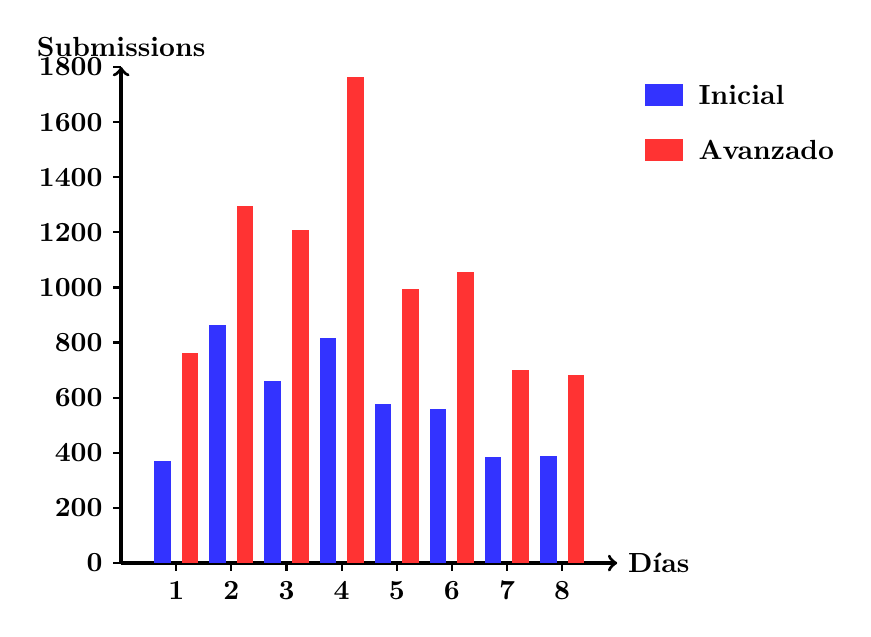
\begin{tikzpicture}[scale=0.7]
% Define coordinates for submissions (Inicial/Avanzado)
% Day 1: Inicial-1 (370), Avanzado-1 (763)
% Day 2: Inicial-2 (863), Avanzado-2 (1295)
% Day 3: Inicial-3 (661), Avanzado-3 (1208)
% Day 4: Inicial-4 (815), Avanzado-4 (1762)
% Day 5: Inicial-5 (578), Avanzado-5 (993)
% Day 6: Inicial-6 (559), Avanzado-6 (1056)
% Day 7: Inicial-7 (384), Avanzado-7 (700)
% Day 8: Inicial-8 (388), Avanzado-8 (681)

% Y-axis (submissions) - goes up to 1800 with jumps of 200
\draw[->,very thick] (0,0) -- (0,9) node[above] {\textbf{Submissions}};
\foreach \y/\label in {0/0, 1/200, 2/400, 3/600, 4/800, 5/1000, 6/1200, 7/1400, 8/1600, 9/1800} {
    \draw[thick] (0,\y) -- (-0.15,\y) node[left] {\textbf{\label}};
}

% X-axis (days) - simplified to just show day numbers
\draw[->,very thick] (0,0) -- (9,0) node[right] {\textbf{Días}};
\foreach \x in {1,2,3,4,5,6,7,8} {
    \draw[thick] (\x,0) -- (\x,-0.15) node[below] {\textbf{\x}};
}

% Bars for Inicial submissions (blue) - using original data values scaled to fit
\fill[blue!80] (0.6,0) rectangle (0.9,1.85);  % 370
\fill[blue!80] (1.6,0) rectangle (1.9,4.315); % 863
\fill[blue!80] (2.6,0) rectangle (2.9,3.305); % 661
\fill[blue!80] (3.6,0) rectangle (3.9,4.075); % 815
\fill[blue!80] (4.6,0) rectangle (4.9,2.89);  % 578
\fill[blue!80] (5.6,0) rectangle (5.9,2.795); % 559
\fill[blue!80] (6.6,0) rectangle (6.9,1.92);  % 384
\fill[blue!80] (7.6,0) rectangle (7.9,1.94);  % 388

% Bars for Avanzado submissions (red) - using original data values scaled to fit
\fill[red!80] (1.1,0) rectangle (1.4,3.815);  % 763
\fill[red!80] (2.1,0) rectangle (2.4,6.475);  % 1295
\fill[red!80] (3.1,0) rectangle (3.4,6.04);   % 1208
\fill[red!80] (4.1,0) rectangle (4.4,8.81);   % 1762
\fill[red!80] (5.1,0) rectangle (5.4,4.965);  % 993
\fill[red!80] (6.1,0) rectangle (6.4,5.28);   % 1056
\fill[red!80] (7.1,0) rectangle (7.4,3.5);    % 700
\fill[red!80] (8.1,0) rectangle (8.4,3.405);  % 681

% Legend - with colored rectangles and text labels
\fill[blue!80] (9.5,8.3) rectangle (10.2,8.7);
\node[right] at (10.3,8.5) {\textbf{Inicial}};
\fill[red!80] (9.5,7.3) rectangle (10.2,7.7);
\node[right] at (10.3,7.5) {\textbf{Avanzado}};

\end{tikzpicture}
\end{center}
\end{frame}

\begin{frame}{Análisis de Submissions}

% Pie charts for Lenguajes Utilizados and Respuestas del Juez

\begin{columns}[t]
\column{0.5\textwidth}
\textbf{Lenguajes Utilizados:}

\vspace{0.2cm}

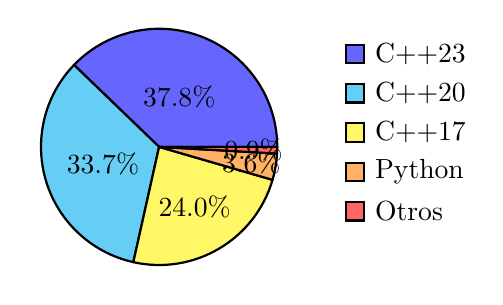
\begin{tikzpicture}
\pie[text=legend, radius=1.5, sum=auto, after number=\%]
  {37.8/C++23, 33.7/C++20, 24.0/C++17, 3.6/Python, 0.9/Otros}
\end{tikzpicture}

\column{0.5\textwidth}
\textbf{Respuestas del Juez:}

\vspace{0.2cm}

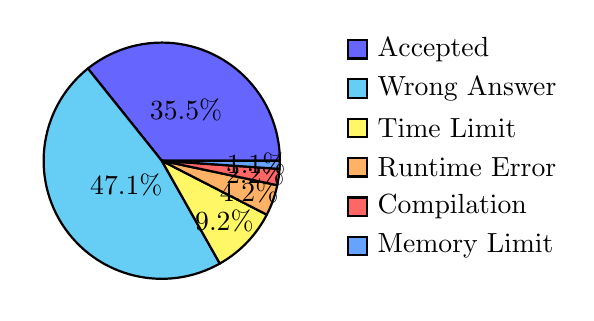
\begin{tikzpicture}
\pie[text=legend, radius=1.5, sum=auto, after number=\%]
  {35.5/Accepted, 47.1/Wrong Answer, 9.2/Time Limit, 4.2/Runtime Error, 2.2/Compilation, 1.1/Memory Limit}
\end{tikzpicture}
\end{columns}


\end{frame}

\begin{frame}{Estadísticas Adicionales}
\begin{center}
\Large
\textbf{Más Información de Submissions}

\vspace{0.3cm}

\begin{columns}[t]
\column{0.5\textwidth}
\textbf{Participación por Contest:}

\vspace{0.1cm}

\small
\begin{itemize}
\item \textbf{Más Participantes:} Avanzado-4 (136)
\item \textbf{Más Submissions:} Avanzado-4 (1,762)
\item \textbf{Promedio Submissions:} 817 por contest
\item \textbf{Participantes Únicos:} 262 total
\end{itemize}

\column{0.5\textwidth}
\textbf{Métricas de Rendimiento:}

\vspace{0.1cm}

\small
\begin{itemize}
\item \textbf{Submissions/Participante:} 49.9 promedio
\item \textbf{Mejor Contest Inicial:} Inicial-8 (51.3\% accepted)
\item \textbf{Contest Más Difícil:} Avanzado-4 (25.8\% accepted)
\item \textbf{Problemas Intentados:} 11-14 por contest
\end{itemize}
\end{columns}


\end{center}
\end{frame}

\begin{frame}{Total de Submissions}
\begin{center}
\Huge
\textbf{¡13,076 SUBMISSIONS!}

\vspace{0.7cm}

\Large
\textbf{En 16 contests durante 8 días}

\vspace{0.3cm}

\normalsize
\begin{itemize}
\item \textbf{262 participantes únicos}
\item \textbf{8 países representados}
\item \textbf{200 problemas disponibles}
\item \textbf{148 problemas únicos}
\end{itemize}

\vspace{0.7cm}

\textbf{¡Gracias por hacer del Training Camp 2025 un éxito rotundo!}
\end{center}
\end{frame}


\section{y ahora... los premios}

\begin{frame}{Vino mucha gente de Tucumán}
\begin{center}
\Large
\textbf{¡Vino mucha gente de Tucumán!}

\vspace{1cm}

\fcolorbox{blue}{blue}{
\includegraphics[width=0.4\textwidth,keepaspectratio]{logos/unt_logo.png}}

\vspace{1cm}

\normalsize
\textbf{Universidad Nacional de Tucumán}

\vspace{0.5cm}

¡Gracias por su participación!
\end{center}
\end{frame}

\begin{frame}{SPOILER ALERT}
\begin{center}
\Huge
\textbf{SPOILER ALERT}

\vspace{2cm}

\Large
¡Algo importante está por venir!
\end{center}
\end{frame}

\begin{frame}{TC 2026?}
\begin{center}
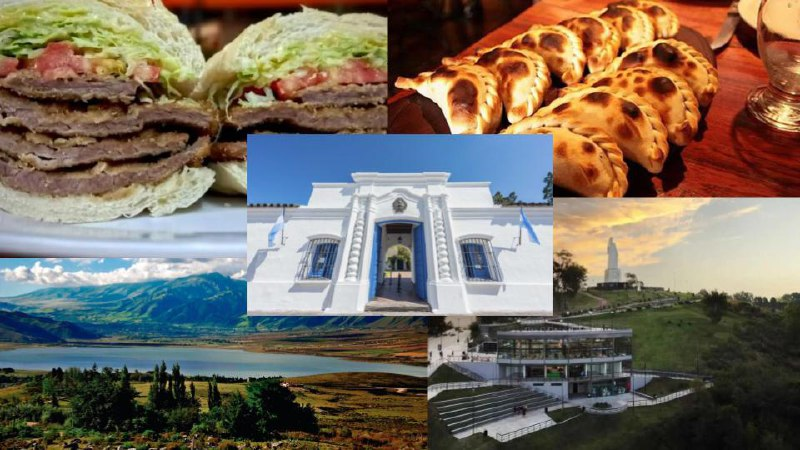
\includegraphics[width=0.98\textwidth,height=0.9\textheight,keepaspectratio]{img/tucu.jpeg}
\end{center}
\end{frame}

% New frame: ahora si, premios
\begin{frame}{ahora si, premios}
    \begin{itemize}
        \item Se entregan premios a los \textbf{top 12} de cada ranking general en el grupo de Codeforces "Training Camp 2025".
        \item Si alguno de los premiados no estuvo presencial, el premio pasa al siguiente en el ranking.
    \end{itemize}
\end{frame}

% New frame: Ranking Inicial
\begin{frame}{Ranking Inicial}
    \begin{columns}
        \column{0.5\textwidth}
        \centering
        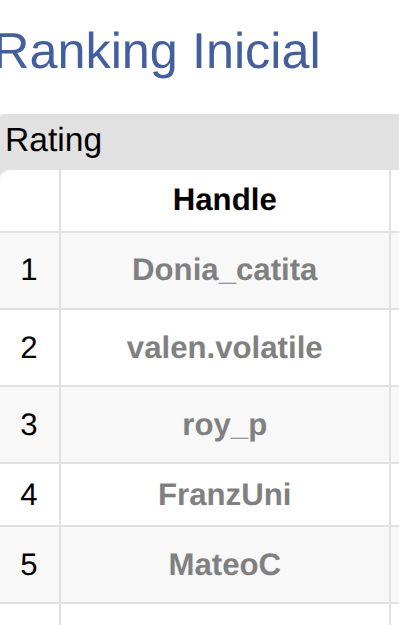
\includegraphics[width=0.7\textwidth,keepaspectratio]{img/inicial-1.png}
        \column{0.5\textwidth}
        \centering
        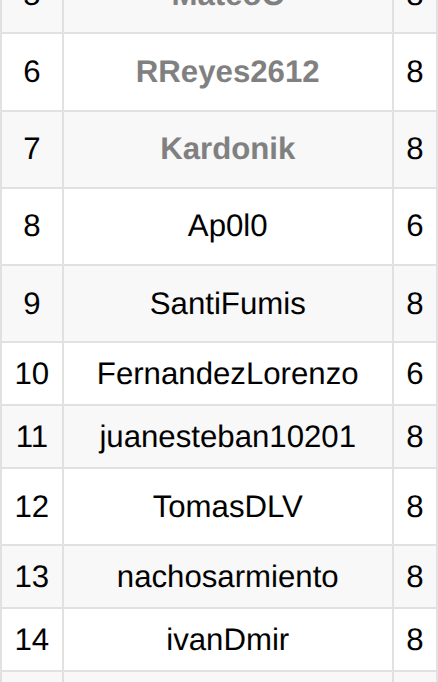
\includegraphics[width=0.7\textwidth,keepaspectratio]{img/inicial-2.png}
    \end{columns}
\end{frame}

% New frame: Ranking Avanzado
\begin{frame}{Ranking Avanzado}
    \begin{columns}
        \column{0.5\textwidth}
        \centering
        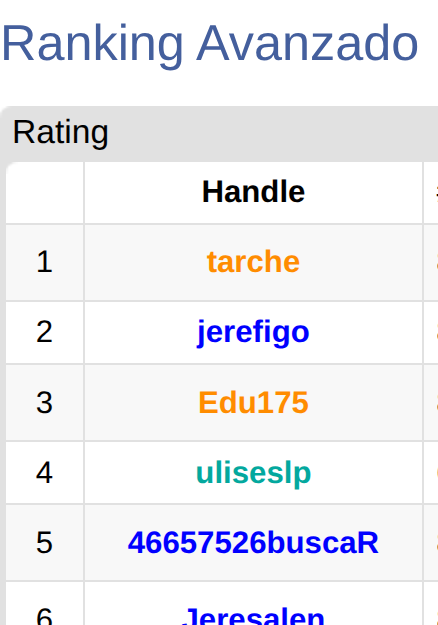
\includegraphics[width=0.7\textwidth,keepaspectratio]{img/avanzado-1.png}
        \column{0.5\textwidth}
        \centering
        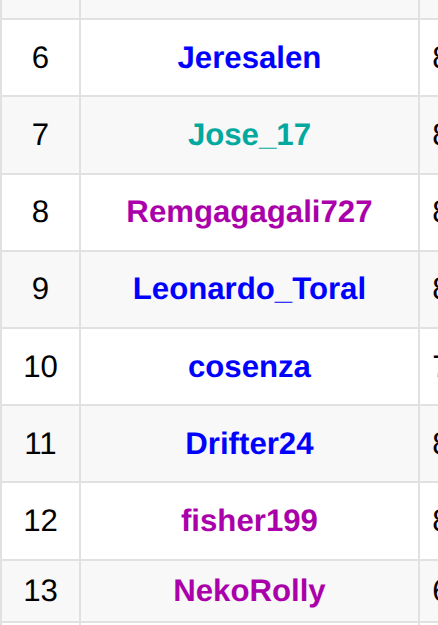
\includegraphics[width=0.7\textwidth,keepaspectratio]{img/avanzado-2.png}
    \end{columns}
\end{frame}


\section{y que hago con todo lo que aprendi?}

\begin{frame}{y que hago con todo lo que aprendi?}
    \begin{center}
        
\includegraphics[width=0.45\textwidth,keepaspectratio]{img/qr-code-aapc.png}

        \vspace{0.5cm}
        {\small
        \textbf{¡Hacete socio/a de la AAPC!}\\
        Apoyá la programación competitiva en Argentina.\\
        \href{https://icpc.com.ar/socios/}{https://icpc.com.ar/socios/}
        }
    \end{center}
\end{frame}

\begin{frame}{Maratona Feminina de Programação (MFP) - Información General}
\begin{center}

\includegraphics[width=0.2\textwidth,keepaspectratio]{img/mfp_logo.jpeg}

\vspace{0.3cm}

\Large
\textbf{Maratona Feminina de Programação}

\vspace{0.2cm}

\normalsize
\textbf{Competencia exclusiva para mujeres en programación}

\vspace{0.3cm}

\begin{itemize}
\item \textbf{Objetivo:} Promover la participación femenina en programación competitiva
\item \textbf{Formato:} Competencia individual o en equipos
\item \textbf{Duración:} 5 horas de competencia intensiva
\item \textbf{Lenguajes:} C/C++, Python, Java, entre otros
\item \textbf{Organización:} Sociedad Brasileña de Computación (SBC)
\end{itemize}

\vspace{0.3cm}

\textbf{¡Una oportunidad única para demostrar tu talento!}

\vspace{0.2cm}

\small
\url{https://www.instagram.com/mfp.sbc}
\end{center}
\end{frame}

\begin{frame}{Maratona Feminina de Programação (MFP) - Beneficios y Participación}
\begin{center}
\Large
\textbf{¿Por qué participar en MFP?}

\vspace{0.1cm}

\normalsize
\begin{itemize}
\item \textbf{Networking:} Conoce a otras programadoras apasionadas
\item \textbf{Desarrollo:} Mejora tus habilidades de resolución de problemas
\item \textbf{Visibilidad:} Demuestra tu talento en la comunidad
\item \textbf{Mentoría:} Acceso a mentoras experimentadas
\item \textbf{Oportunidades:} Puertas abiertas a competencias internacionales
\end{itemize}

\vspace{0.1cm}

\textbf{¡Rompe barreras y construye tu futuro en tecnología!}

\normalsize
\textbf{Próxima edición:} Consulta las fechas en sus redes sociales

\small
\url{https://www.instagram.com/mfp.sbc}
\end{center}
\end{frame}

\begin{frame}{Torneo Argentino de Programación (TAP) - Información General}
\begin{center}

\includegraphics[width=0.2\textwidth,keepaspectratio]{img/tap_logo.png}

\vspace{0.1cm}

\Large
\textbf{15º Torneo Argentino de Programación 2025}

\normalsize
\textbf{Sábado 23 de agosto de 2025}

\vspace{0.1cm}

\begin{itemize}
\item \textbf{Competencia:} 5 horas de duración
\item \textbf{Equipos:} 3 personas por equipo (1 PC)
\item \textbf{Lenguajes:} C/C++, Python, Java o Kotlin
\item \textbf{Requisito:} Ser estudiante de educación superior en Argentina
\item \textbf{Clasificación:} Para ICPC Latinoamérica (Chile 2026)
\end{itemize}

\textbf{¡Inscripción hasta el 20 de agosto!}

\small
\url{https://icpc.global/regionals/finder/TAP-2026}
\end{center}
\end{frame}

\begin{frame}{Torneo Argentino de Programación (TAP) - Sedes de Competencia}
\begin{center}
\Large
\textbf{Sedes de Competencia 2025}

\vspace{0.2cm}

\normalsize
\begin{columns}[t]
\column{0.5\textwidth}
\small
\begin{itemize}
\item \textbf{UNJu} (Jujuy)
\item \textbf{UNSa} (Nueva Orán, Salta)
\item \textbf{UNT} (Tucumán)
\item \textbf{UNdeC} (La Rioja)
\item \textbf{FAMAF-UNC} (Córdoba)
\item \textbf{UNRC} (Córdoba)
\item \textbf{UTN Santa Fe}
\end{itemize}

\column{0.5\textwidth}
\small
\begin{itemize}
\item \textbf{UNLAM} (Bs. As.)
\item \textbf{UNLP} (Bs. As.)
\item \textbf{Inst. Balseiro} (Río Negro)
\item \textbf{UTN Resistencia} \textbf{¡Nueva sede!}
\end{itemize}

\end{columns}

\vspace{0.2cm}

\textbf{¡Tu universidad puede ser sede!}

\normalsize
Solo necesitás conexión a internet

\small
\url{https://icpc.com.ar/tap}
\end{center}
\end{frame}

\begin{frame}{Regional Sudamérica-Sur}
\begin{center}
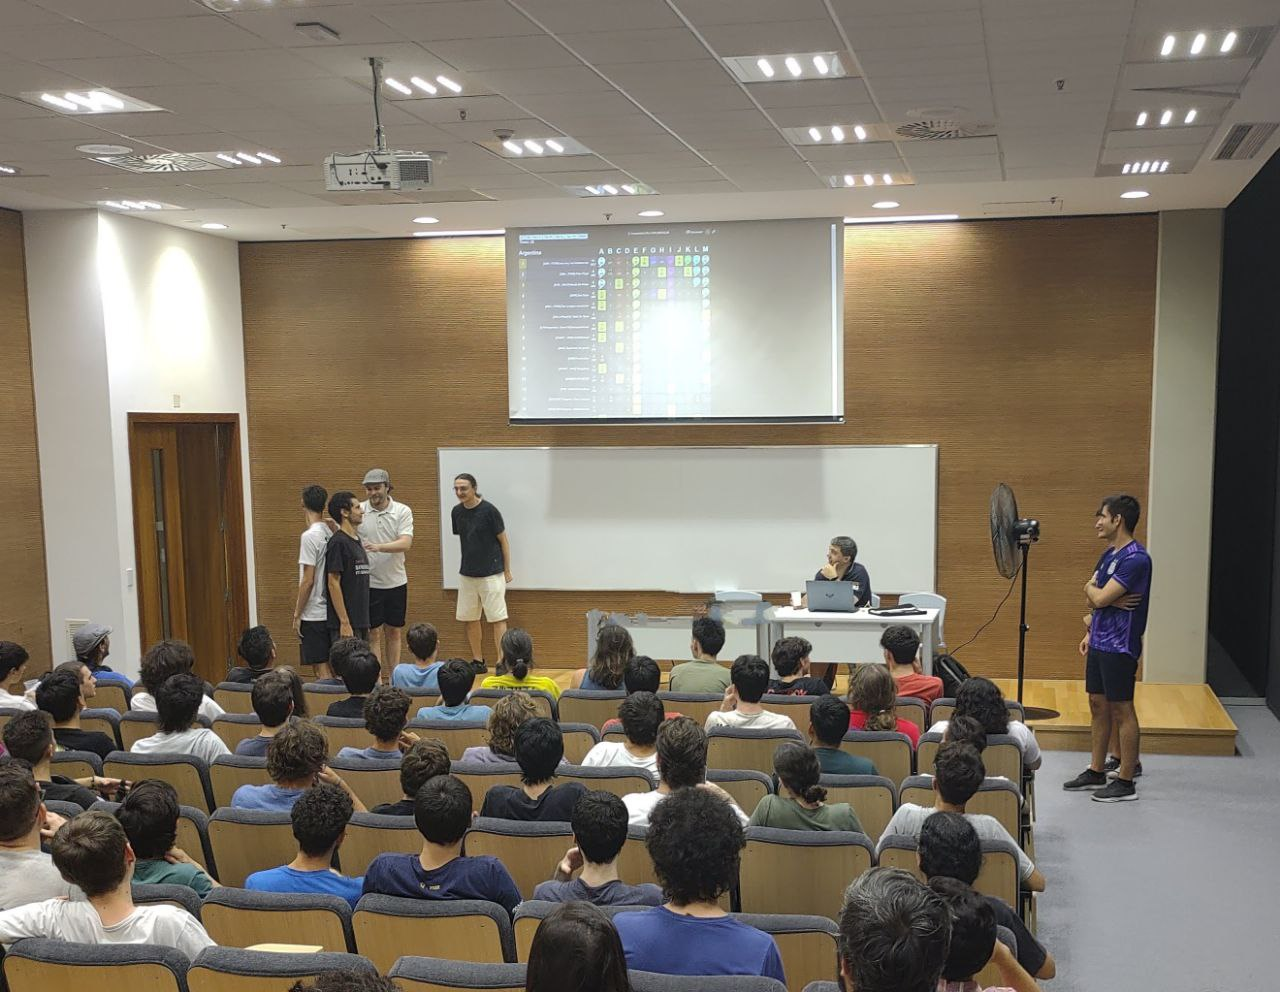
\includegraphics[width=0.3\textwidth,keepaspectratio]{img/regional_logo.jpg}

\vspace{0.2cm}

\Large
\textbf{Regional Sudamérica-Sur 2025}

\vspace{0.1cm}

\normalsize
\textbf{8 de noviembre de 2025}

\vspace{0.1cm}

\begin{itemize}
\item \textbf{Participantes:} Equipos clasificados del TAP y otros países
\item \textbf{Países:} Argentina, Chile, Uruguay, Paraguay, Bolivia
\item \textbf{Formato:} 5 horas de competencia intensiva
\item \textbf{Premio:} Clasificación a PDA 2026
\end{itemize}

\vspace{0.1cm}

\textbf{¡El siguiente paso después del TAP!}

\small
\url{https://icpc.com.ar/regional-latinoamericana}
\end{center}
\end{frame}

\begin{frame}{Programadores de América 2026}
\begin{center}

\vspace{0.2cm}

\normalsize
\textbf{Santiago de Chile, Marzo 2026}

\vspace{0.2cm}


\includegraphics[width=0.5\textwidth,keepaspectratio]{img/pda_chile.png}

\vspace{0.3cm}

\begin{itemize}
\item \textbf{Competencia:} Final continental de programación
\item \textbf{Participantes:} Mejores equipos de Latinoamérica
\item \textbf{Formato:} 5 horas de competencia intensiva
\item \textbf{Premio:} Clasificación a la Final Mundial ICPC 2026
\end{itemize}

\vspace{0.2cm}

\textbf{¡La meta final de todo programador competitivo!}

\small
\url{https://icpc.global}
\end{center}
\end{frame}


\section{Gracias a todos}

\begin{frame}{Gracias Disertantes}
    \begin{itemize}
        \item Federico Quijada
        \item Juan Pablo Cabaña
        \item Mariano Feresin
        \item Facundo Gutierrez
        \item Agustín Santiago Gutiérrez
        \item Mateo Carranza Velez
        \item Federico Bersano
        \item Lautaro Lasorsa
        \item Franco De Rico
        \item Ivo Pajor
        \item Carlos Miguel Soto
        \item Sebastián Mestre
    \end{itemize}
\end{frame}

% Add a frame for Gracias Setters with colorized handles
\begin{frame}{Gracias Setters}
    \begin{itemize}
        \item {\color{purple} CodigoL}
        \item {\color{orange} MateoCV}
        \item {\color{orange} elsantodel90}
        \item {\color{orange} lsantire}
        \item {\color{orange} Heibor}
        \item {\color{orange} MarcosK}
        \item {\color{cyan} Aristides}
    \end{itemize}
\end{frame}

% Add a frame for Gracias Voluntarios
\begin{frame}{Gracias Voluntarios}
    \begin{center}
        Vicky C, Vicky P, Eli, Fran, Bauti y Felipe.

        \vspace{0.5cm}
        Hacedores del coffee-break y ayuda para que todo salga bien.

        \vspace{0.7cm}
        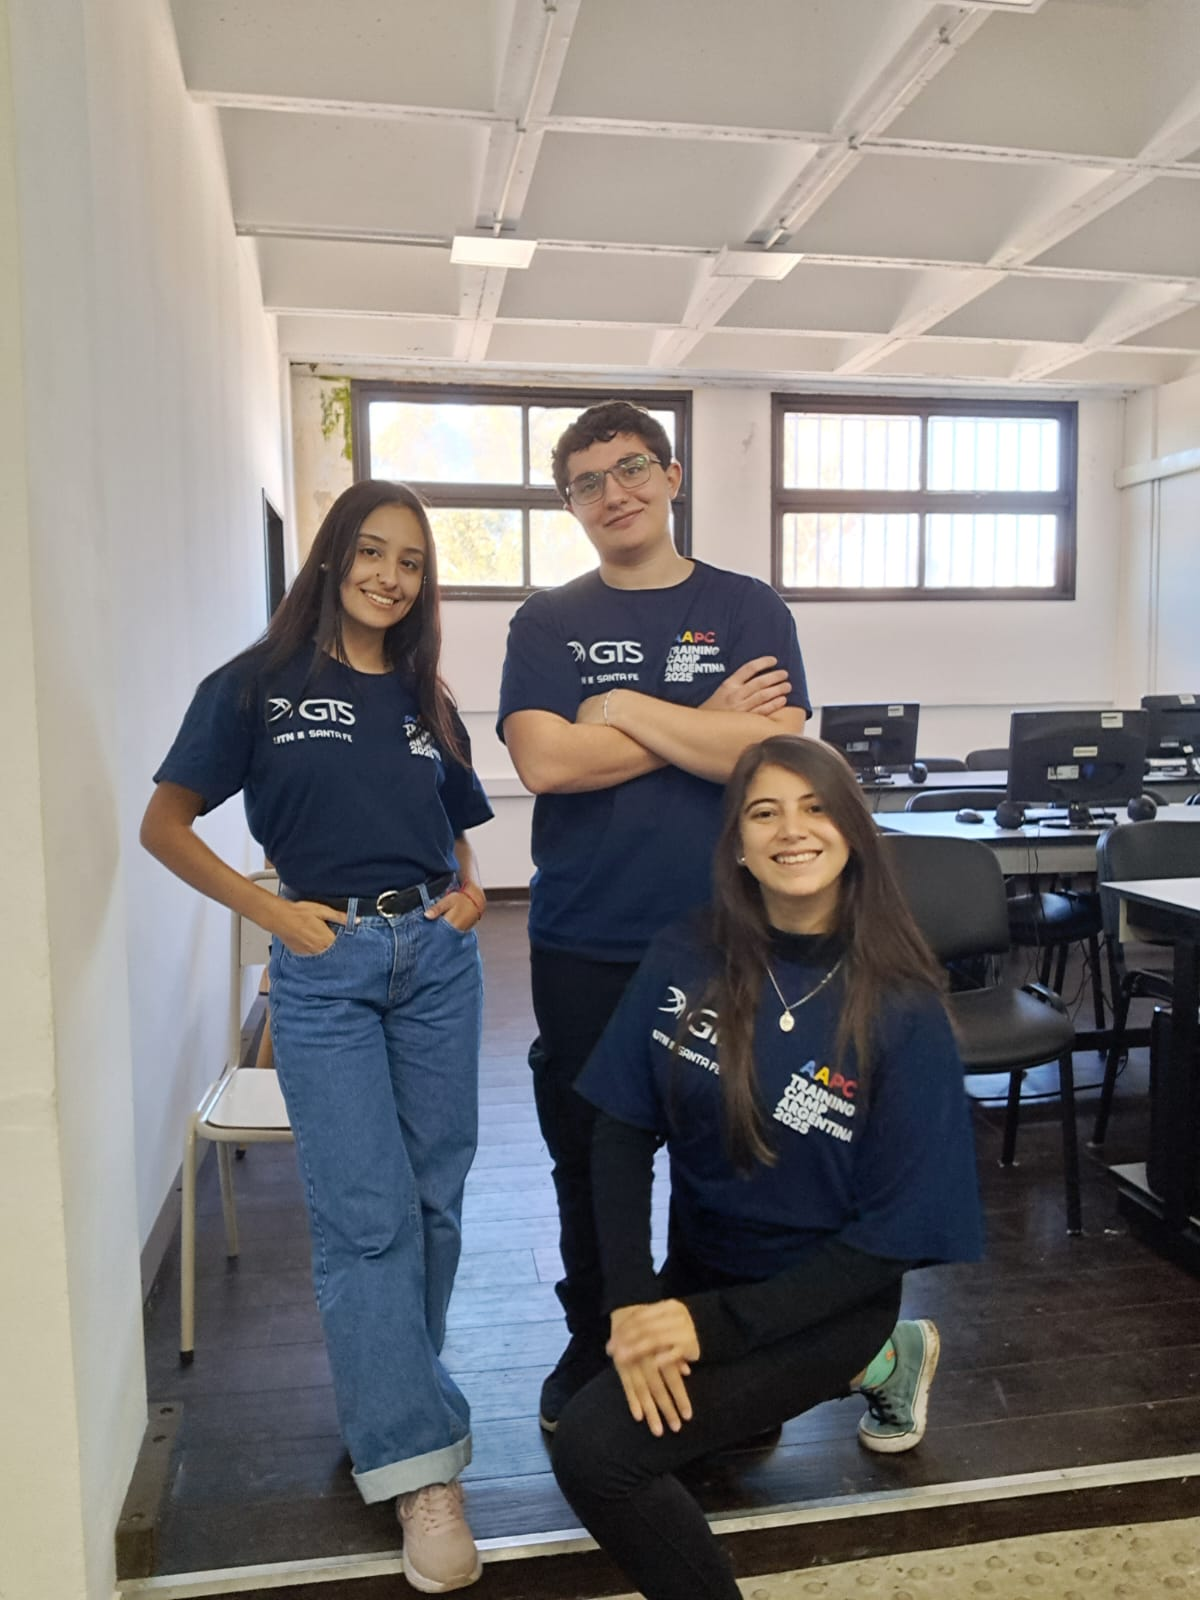
\includegraphics[width=0.5\textwidth,keepaspectratio,trim=0cm 10cm 0cm 10cm,clip]{img/voluntarios.jpeg}
    \end{center}
\end{frame}

% Add a frame for Gracias UTN-FRSF
\begin{frame}{Gracias UTN-FRSF}
    \begin{center}
        
\includegraphics[width=1.05\textwidth,keepaspectratio]{logos/utn_santafe.png}

        \vspace{0.5cm}
        Equipo de Soporte, Mantenimiento, Limpieza, etc.
    \end{center}
\end{frame}

% Add a frame for Gracias a ustedes
\begin{frame}{Gracias a ustedes}
    \begin{center}
        \includegraphics[width=0.7\textwidth,keepaspectratio]{img/evento-gts.JPG}

        \vspace{0.5cm}
        nos vemos en TC 2026?
    \end{center}
\end{frame}

\end{document}